\documentclass[10pt,letterpaper]{datasheet}

\usepackage{amssymb}
\usepackage{color}
\usepackage[]{graphicx}
\usepackage{lipsum}
\usepackage{multicol}
\usepackage[small]{subfigure}
\usepackage{tabularx}

\newlength\SUBSIZE
\newcommand{\epic}{Epic~}


\pagestyle{fancy}
  \lfoot[]{}
  \cfoot[]{HiJack Datasheet -- Rev. A}

\usepackage{hyperref}
\hypersetup{pdftitle={HiJack Datasheet},
  pdfauthor={Thomas Schmid \& Prabal Dutta},
  pdfkeywords={hijack,phone,ios}}

\begin{document}
\title{\color{blue}{\bf HiJack}}
\author{Thomas Schmid \& Prabal Dutta}
\date{}
\maketitle
\makefooter
\thispagestyle{fancy}

\section*{Product Description}
\begin{multicols}{2}
HiJack is a hardware/software platform for creating cubic-inch sensor
peripherals for the mobile phone. HiJack devices harvest power and use
bandwidth from the mobile phone's headset interface. The HiJack platform
enables a new class of small and cheap phone-centric sensor peripherals that
support plug-and-play operation. HiJack has been tested with the iPhone
3G/3GS/4G, iPod Touch, and iPad devices.

\subsection*{Data}
The HiJack communications layer offers two data transfer schemes. The first
allows 300 baud data transfer using Bell 202 FSK signaling. The second offers
8.82 kbaud using a Manchester-encoded, direct-digital communication using
hardware accelerators on the HiJack microcontroller and a software-defined,
digital radio modulator/demodulator on the phone. The first scheme is
described in the ISLPED'10 Design Contest entry (below). The second scheme is
described in the DEV'10 paper below.

  \begin{center}
    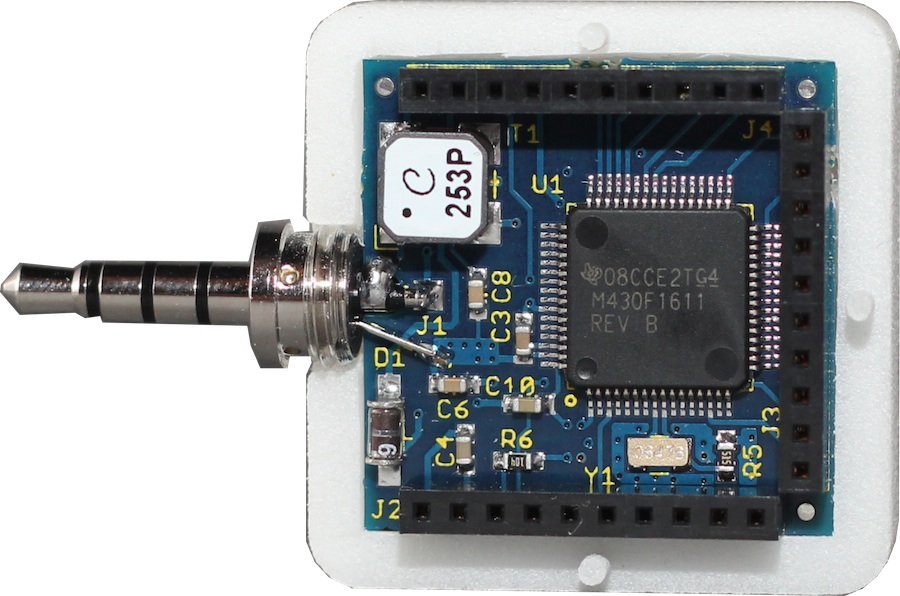
\includegraphics[width=3in]{hijack.jpg}
  \end{center}

\subsection*{Power}
The HiJack energy harvester can supply 7.4~mW to a load with 47\% power
conversion efficiency when driven by a 22~kHz tone from the output from a
single audio channel on the iPhone 3GS headset port. A linear regulators
provides a stable voltage to external deices at 2.75~V.




\end{multicols}


\section*{Highlights}
\begin{multicols}{2}
\begin{itemize}
\item TI MSP430F1611 Mixed-Signal Microcontroller
\item I2C, SPI, UART peripheral interfaces
\item 4x ADC and 2x DAC
\item Timer input and output for capture or PWM
\end{itemize}
\end{multicols}


\section*{Applications}
\begin{multicols}{2}
The HiJack board allows to interface to a myriad of sensorboards including
ozone, carbon monoxide, DVM, blood pressure, blood glucose, and others.  We
successfully interfaced the HiJack board with: (1) a simple demo board with
temperature/humidity sensors, PIR motion sensor, and potentiometer; (2) a
3-lead EKG sensor; (3) a basic soil moisture sensor; (4) a breakout board for
fast prototyping; (5) A RS-232 pass-through using the Maxim 3232 IC.
\end{multicols}

\newpage

\begin{multicols}{2}

\section*{System}

\begin{tabular}{p{0.75in} l}
MCU          & MSP430F1611IRTDT\\
~~Flash      & 48~KB\\
~~RAM        & 10~KB\\
~~Clock      & 4/8~MHz\\
~~Wakeup     & 6~$\mu$s (typ)\\
\\
Regulator    & MIC5231\\
~~Vout       & 2.75~V\\
\end{tabular}

\section*{Mechanical}

\begin{tabular}{p{1.05in} l}

\\
Dimensions     & 25.4 mm x 25.4 mm x 8.7 mm\\
~~~w/jack      & 45.5 mm x 25.4 mm x 8.7 mm\\
\\
Operating Temp & -40 to +85$^\circ$C \\ 
\\
Storage Temp   & -50 to +125$^\circ$C \\
\\
Humidity       & 0 to 99\% RH
\end{tabular}


\section*{Software Support}

\begin{tabular}{p{0.5in} l}

{\tt TinyOS}  & {\tt make hijack [install [miniprog]]}\\
{\tt GNU/GCC} & {\tt msp430-gcc} toolchain\\
{\tt iOS}     & see \url{http://developer.apple.com}\\
\end{tabular}


\section*{Supporting Hardware and Tools}

\begin{tabular}{p{1.05in} l}
Programmer       & USB programmer for the MSP430\\
ProtoBoard       & Simple breakout board\\
\end{tabular}


\section*{References}

Ye-Sheng Kuo, Sonal Verma, Thomas Schmid, and Prabal Dutta, "Hijacking Power and Bandwidth from the Mobile Phone's Audio Interface", First Annual Symposium on Computing for Development (DEV'10), Dec. 2010. 

Ye-Sheng Kuo, Thomas Schmid, and Prabal Dutta, "Hijacking Power and Bandwidth from the Mobile Phone's Audio Interface", International Symposium on Low Power Electronics and Design (ISLPED'10) Design Contest, Aug. 2010. 

\begin{multicols}{2}
\section*{\small{Legal}}

\begin{tiny}

Schmid \& Dutta reserve all rights to this document and the information
contained herein.  Product names, trademarks, or logos described or
displayed herein may be subject to third-party
intellectual property rights.  Permission to use, copy, and distribute
this document, without fee, and without written agreement, is hereby
granted, provided that the document is not modified in any manner.

\vspace{1mm}
\noindent
In no event shall Schmid \& Dutta be liable to any party for direct,
indirect, special, incidental, or consequential damages arising out of
the use of this information or the hardware and software that this
document describes, even if Schmid \& Dutta have been advised of the
possibility of such damage.

\vspace{1mm}
\noindent
Schmid \& Dutta specifically disclaims any warranties, including, but not
limited to, the implied warranties of mechantability and fitness for a
particular purpose.  The information contained herein is provided on
an ``as is'' basis, and Schmid \& Dutta has no obligation to provide
maintenance, support, updates, enhancements, or modifications.  This
document may be revised by Schmid \& Dutta at any time.

\noindent
Copyright \copyright~2009, T. Schmid \& P. Dutta.  All Rights Reserved.
\end{tiny}

\end{multicols}


\end{multicols}
\end{document}

